\documentclass{gescons}

\genre {Resumo do Biênio}
\author{Luziânia Medeiros e~Paulo Abrantes}
\authorrole{Coordenadores da Expedição Paracientífica Expo 2025 Osaka}
\title{Conscienciologia em Expansão: Distribuição de Publicações no Japão e~Europa}

\begin{document}
    \makeentrevistatitle
    %\maketitle

    %\fullwidthimage{fields}{b}

    %\coverart{back/editorial}
    \coverart{../fundo-generico}
    
%    \begin{multicols}{2}

%\begin{center}
%    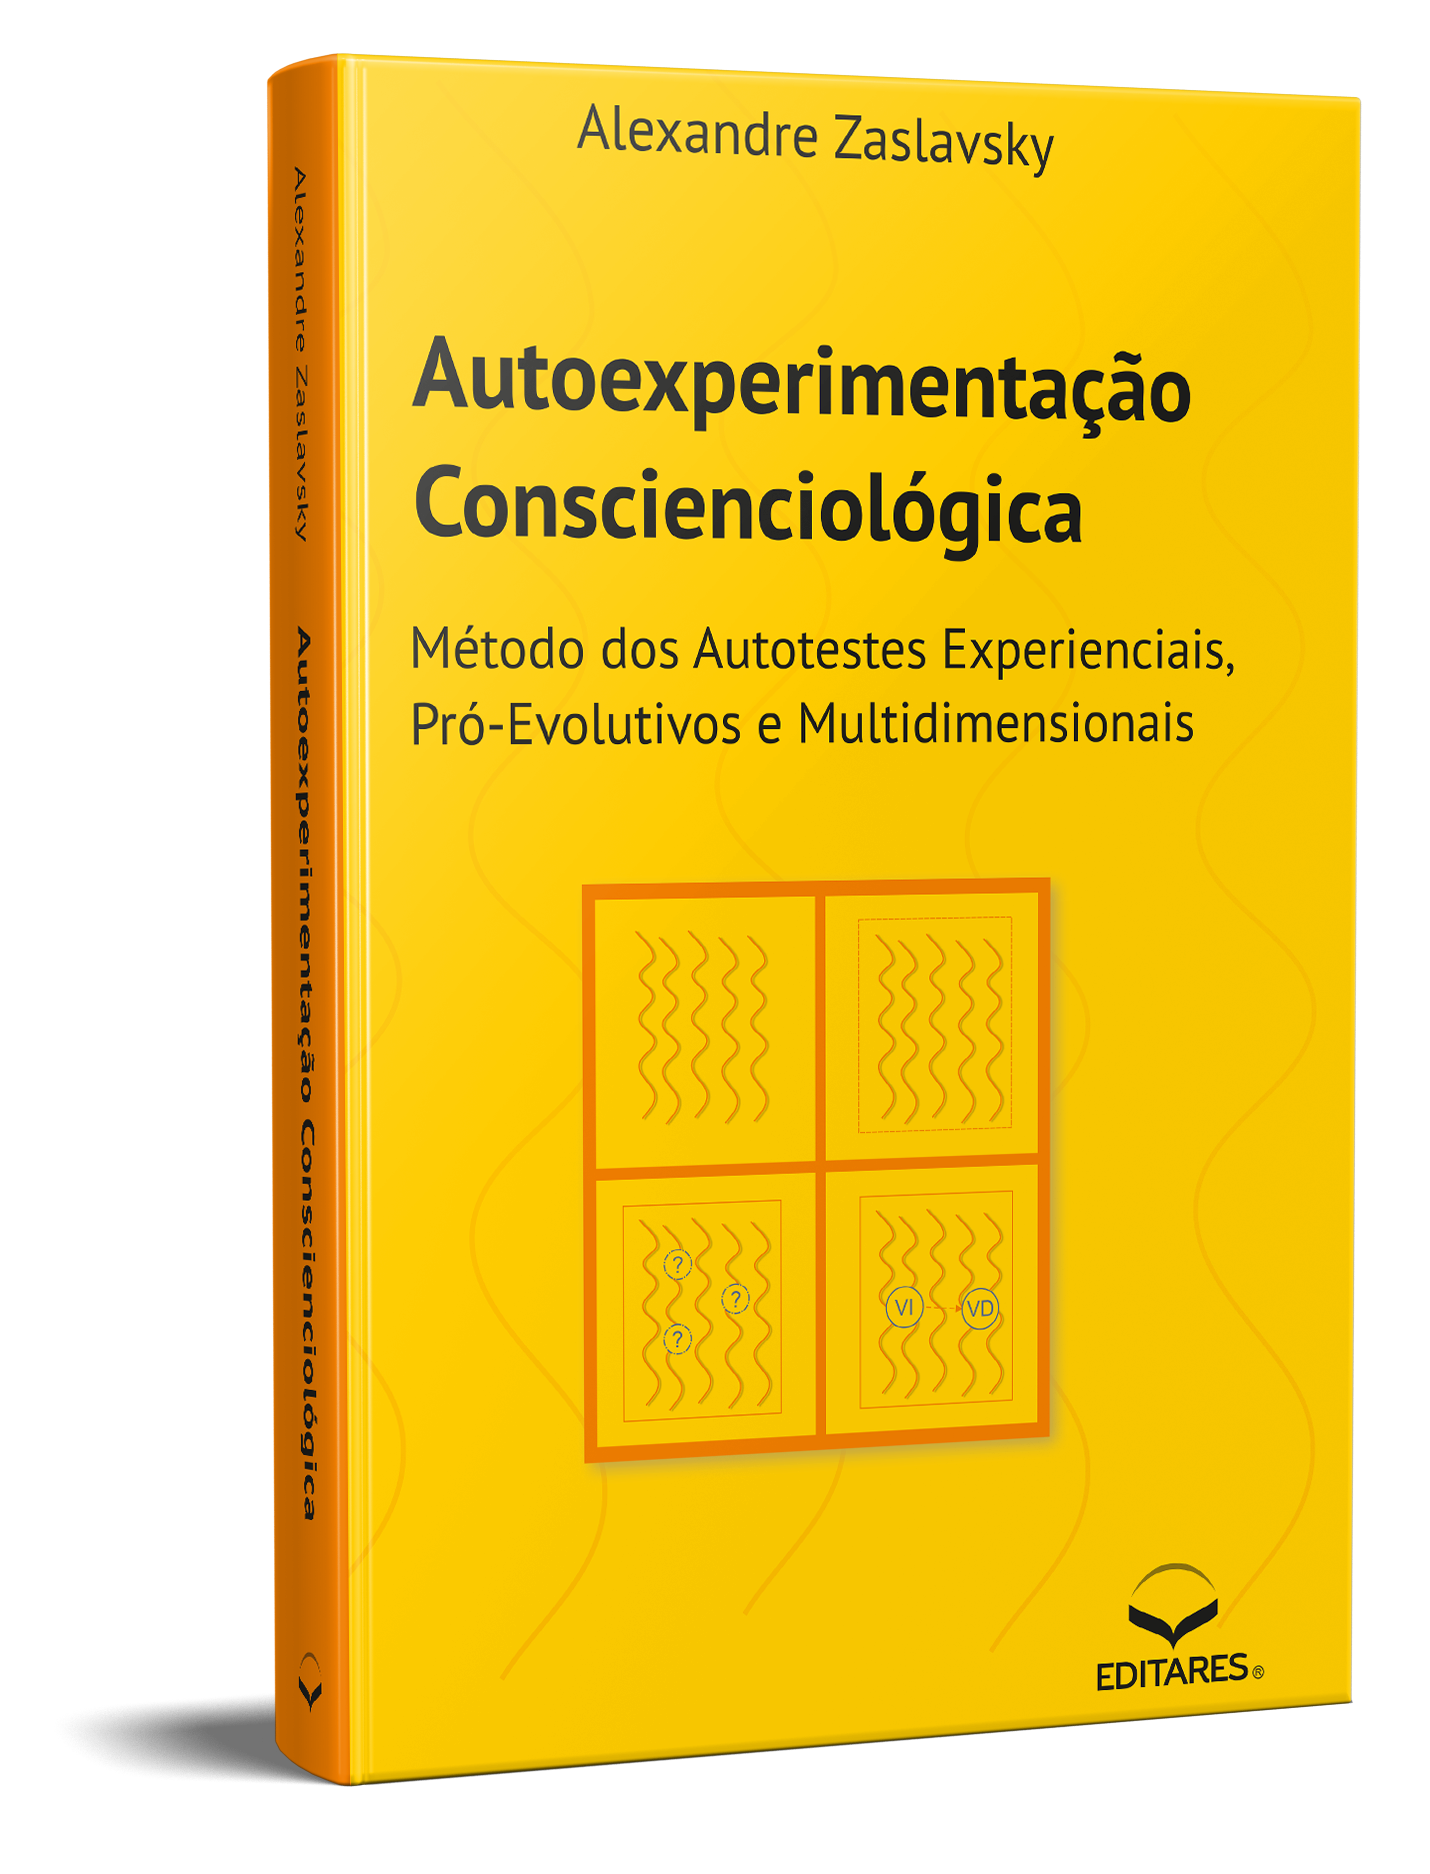
\includegraphics[width=4cm]{articles/entrevista/mockups/Alexandre-Zas}
%\end{center}


% \subsection*{Coordenadores da Expedição Paracientífica Expo 2025 Osaka}

A \emph{Expedição Paracientífica Expo 2025 Osaka} consistiu em viagem técnica de pesquisa grupal, planejada em detalhes durante 2 anos, incluindo instrumentos de registro e~documentação para coleta, sistematização, debate, aprofundamento e~síntese dos achados e~parachados. Tudo isso com o~propósito de refletir sobre o~\emph{Megacentro Cultural Holoteca} no ambiente universalista, pacífico e~multicultural de uma Expo Mundial.

\subsection*{Gestação de publicações}

Para estabelecer a~interlocução com o~público da Expo, identificou-se a~necessidade de apresentar a~Cognópolis, a~neociência Conscienciologia e~seu propositor, as estruturas de pesquisa e~educação, além das principais ações e~projetos, entre eles o~Jovem Pesquisador e~o~Megacentro Cultural Holoteca. Dessa demanda nasceu a~proposta do \emph{Holothecology Supplement,} \textbf{primeira versão} da revista Holotecologia em inglês.

Parte dos integrantes da Expedição estava há 1 ano e~meio desenvolvendo o~dicionário de termos da Conscienciologia em japonês. Foi proposto ao grupo avaliar a~possibilidade de publicar uma edição gratuita com os verbetes já concluídos, em formato de miniglossário, para distribuição entre os japoneses de modo a~presenteá-los com neovocábulos no idioma local. A~equipe da Nipoteca da Holoteca aceitou prontamente o~desafio e~\textbf{fez a~obra acontecer em 2 meses.}

\subsection*{A força do grupo: financiamento e~distribuição das publicações}

% to-do: adicionar imagem japao.jpeg aqui

A produção editorial seguia trabalhando intensamente, mas havia um desafio: viabilizar financeiramente as impressões. Surgiu então a~ideia de arrecadação por meio de um item colecionável e~criou-se uma edição limitada da moeda comemorativa da Expedição. As doações se multiplicaram, e~os recurso obtidos permitiram imprimir \textbf{1000 revistas e~500 mini-glossários.} Essa conquista foi coletiva, totalmente voluntária e~movida pelo propósito de difundir as ideias da Conscienciologia junto a~um público internacional mais amplo.

O material chegou a~tempo de ser levado por pesquisadores que partiam para diferentes países da Europa, em curso itinerante do \emph{Cosmovisão} promovido pela \emph{Associação Internacional de Inversão Existencial} (ASSINVÉXIS). Dezenas de exemplares da revista \emph{Holothecology} foram distribuídos na Inglaterra, França, Áustria e~Suíça. Segundo relatos, a~publicação facilitou diálogos e~conexões em diversos contextos ao longo da viagem. \textbf{A união faz a~força!}



\subsection*{Balanço e~prospectivas}

\begin{wrapfigure}{r}{0.35\textwidth}
  %\begin{left}
  % trim={<left> <lower> <right> <upper>}
  \vspace{-15mm}\hspace{-1mm}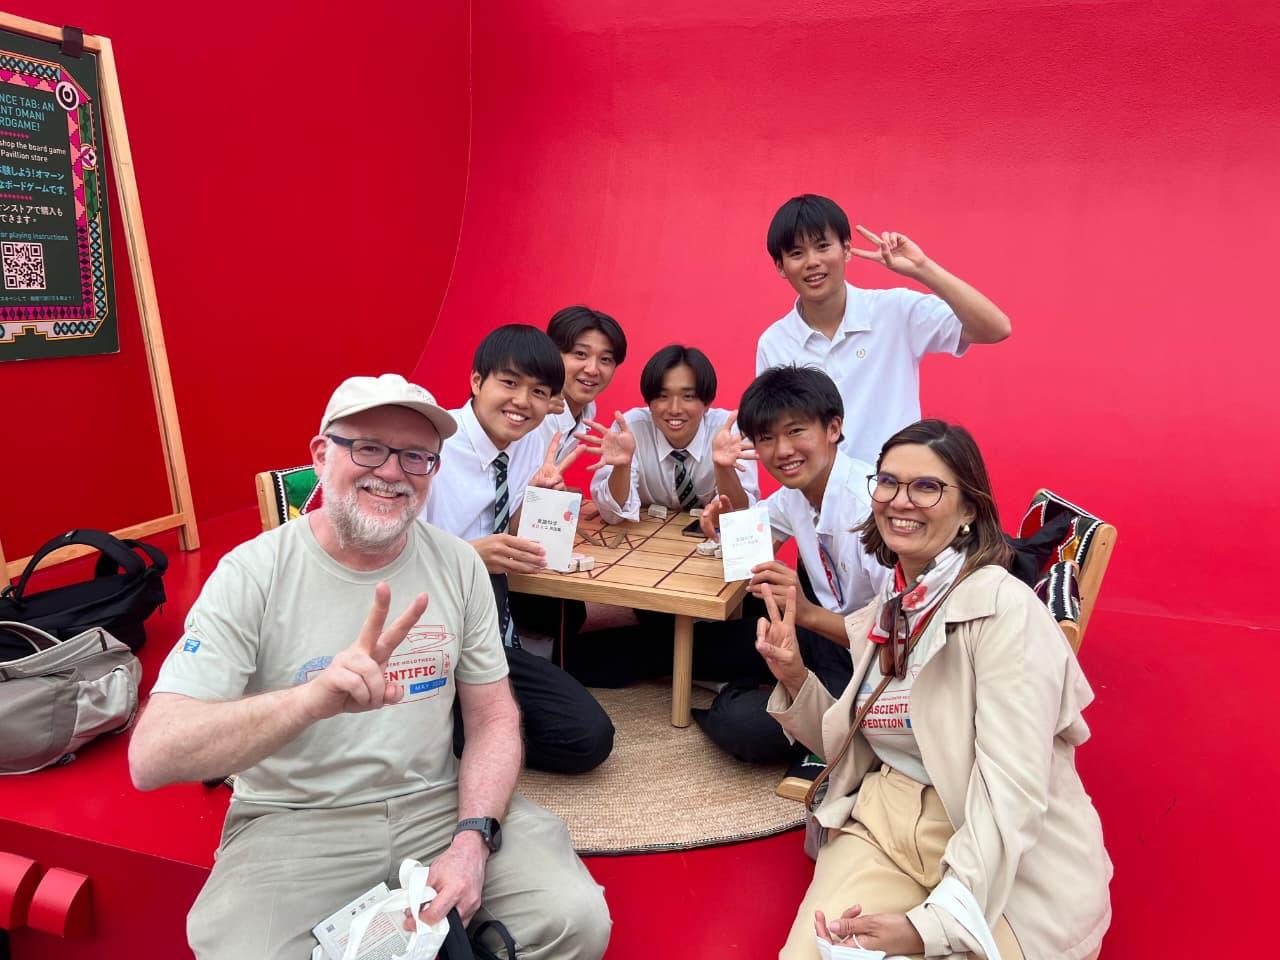
\includegraphics[width=7cm,trim={130 100 105 120},clip]{articles/resumo/fotos/materia3/japao.jpeg}
  %\end{left}
\end{wrapfigure}

No Japão, foram entregues 260 \emph{Miniglossários,} 215 \emph{Holothecology,} 36 \emph{Our Evolution,} 2 \emph{Léxicos de Ortopensatas} e~1 \emph{Manual dos Megapensenes Trivocabulares.} As obras foram deixadas em 8 cidades japonesas, incluindo bibliotecas, sebos, universidades, instituições e~circularam na Expo em pelo menos 43 pavilhões de países dos 5 continentes, além de espaços de organizações internacionais como a~ONU, União Europeia, Cruz Vermelha e~o~Bureau International des Expositions (BIE). Sem falar dos contatos espontâneos com japoneses em locais diversos visitados no Japão e~com visitantes de várias nacionalidades durante a~Expo.

Essas interações estabeleceram novos canais de comunicação e~cooperação com pessoas e~instituições, verdadeiras \textbf{pontes interassistenciais} de natureza variada a~serem cultivadas e~desenvolvidas nos próximos anos.

Tais iniciativas fortalecem e~impulsionam o~avanço do Megacentro Cultural Holoteca, um empreendimento grupal prioritário para a~comunidade conscienciológica, de natureza policármica, abrangente, que contribuirá significativamente para a~consolidação da Conscienciologia no planeta.

%v \textbf{{[}INSERIR FOTOS DA PASTA MATÉRIA 4 - \emph{falta receber essas fotos}{]}}

%\noindent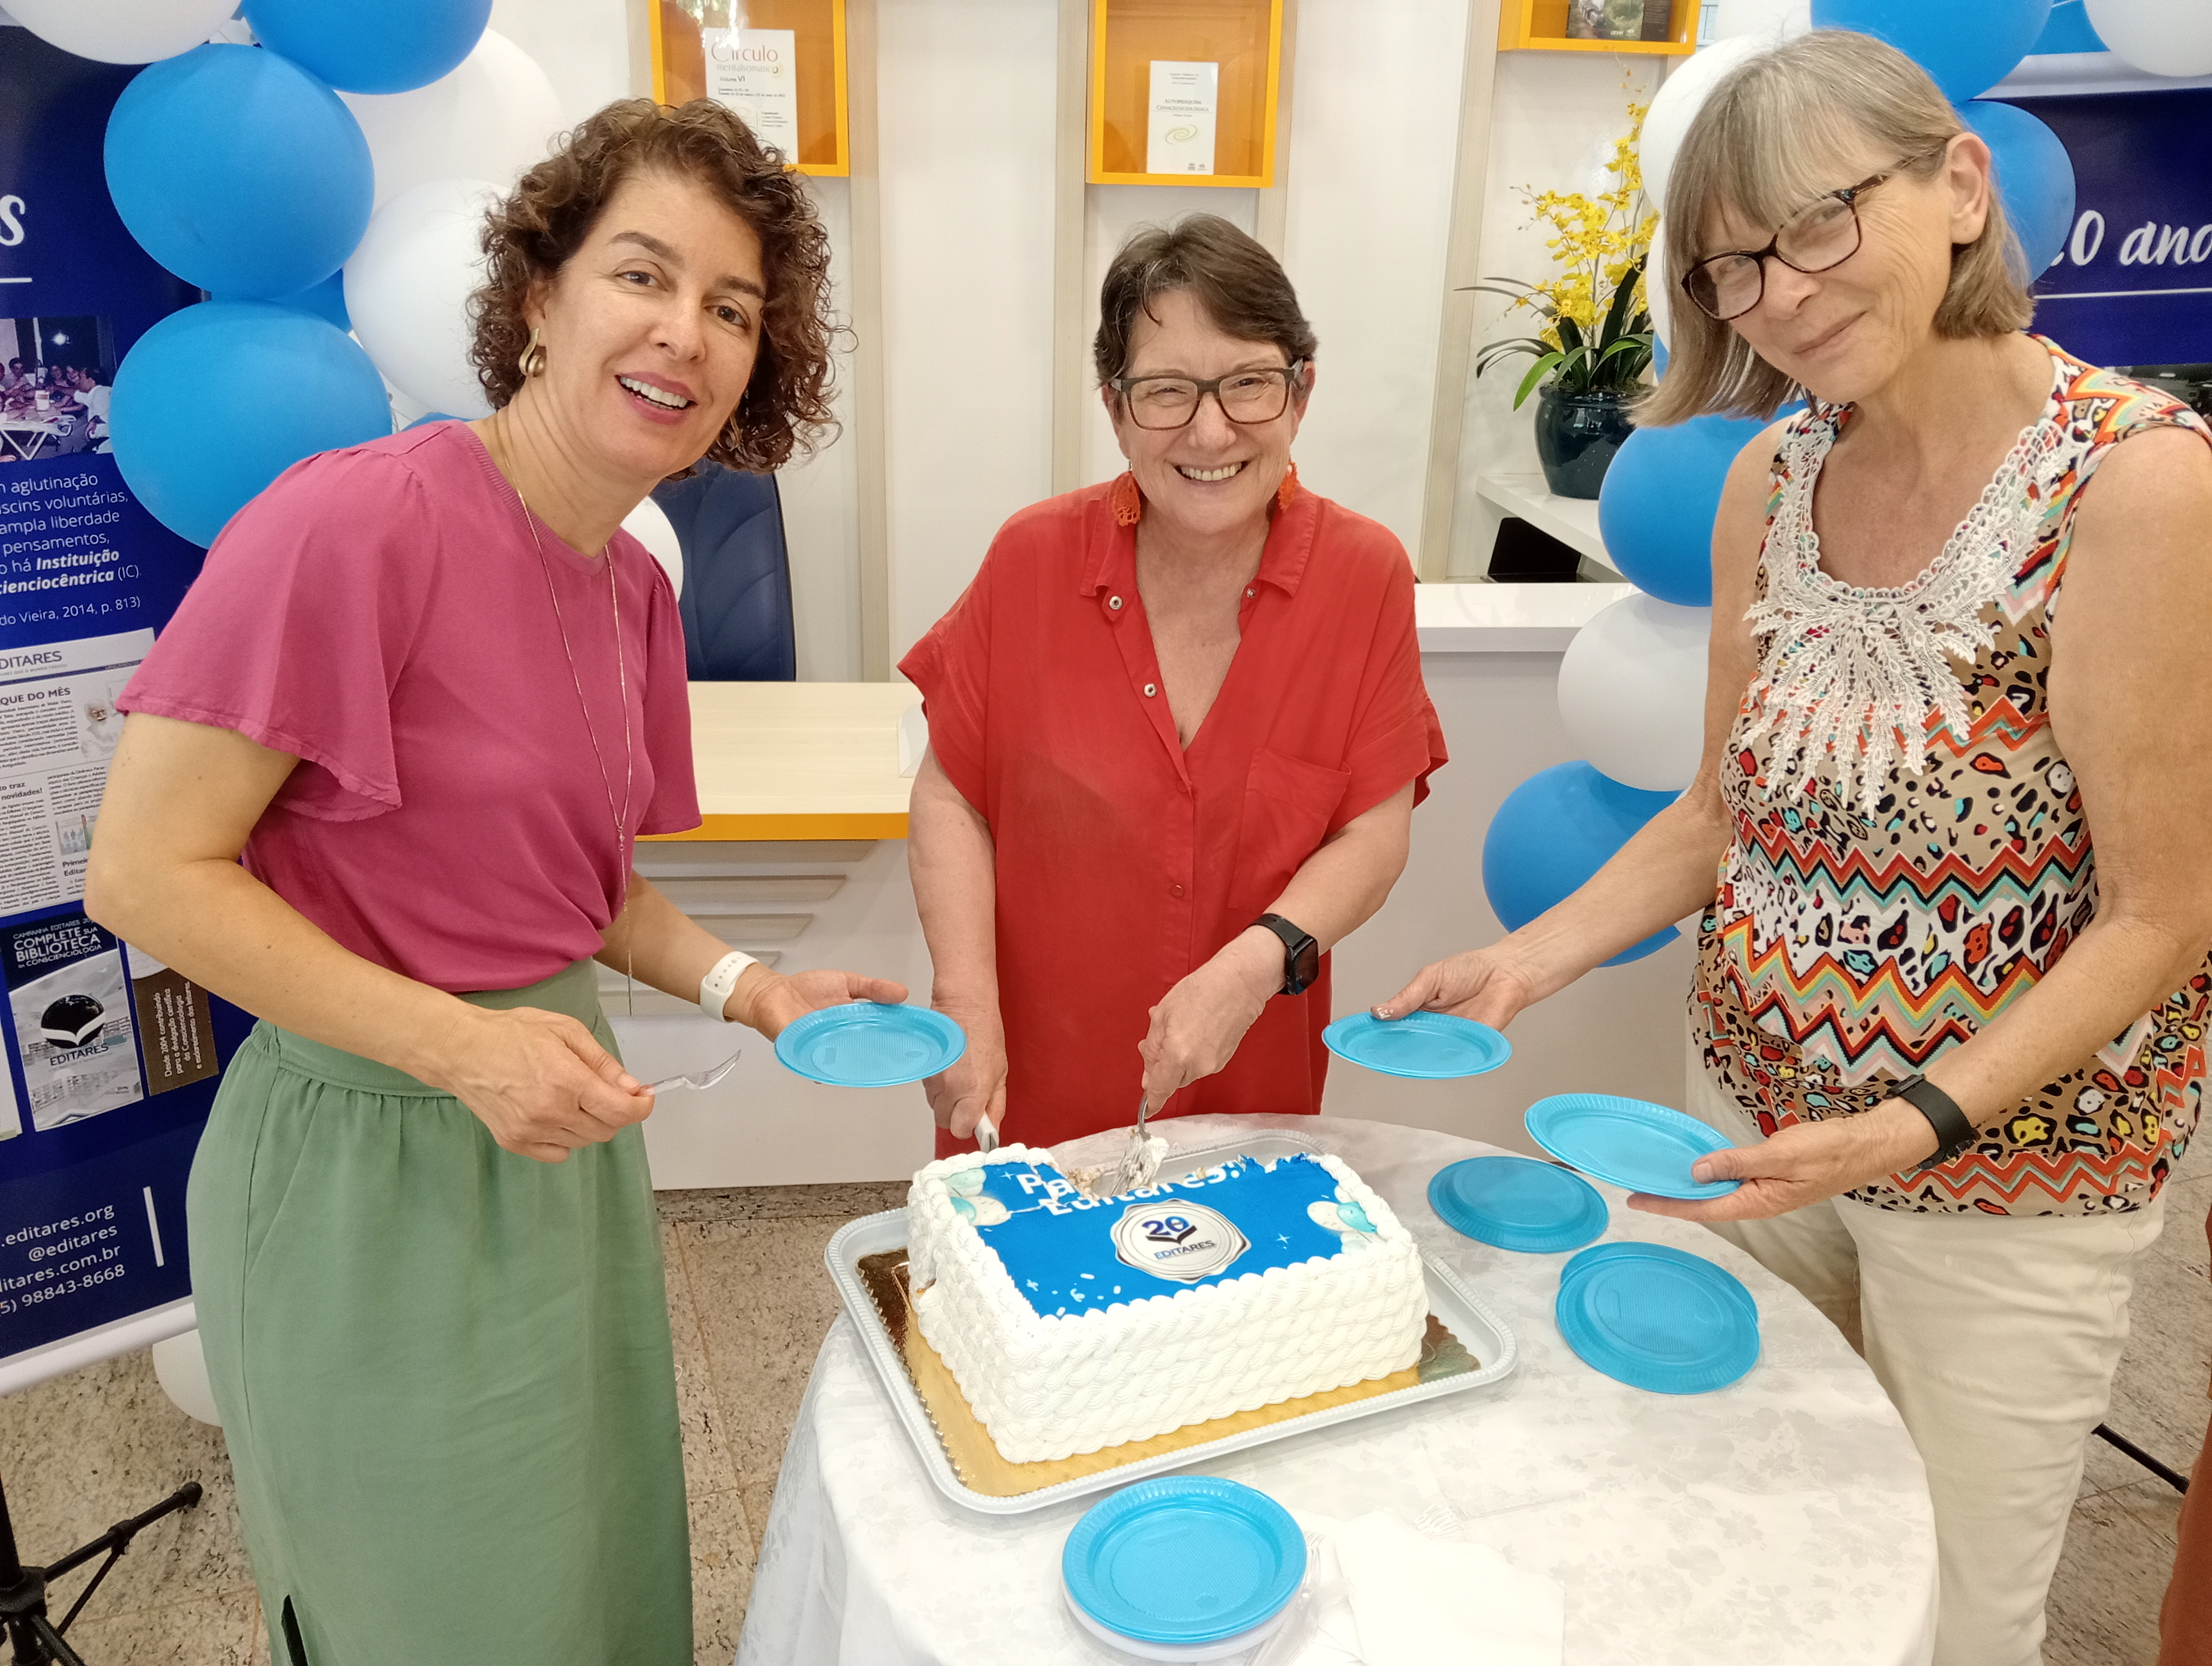
\includegraphics[width=9cm, height=9cm]{articles/resumo/fotos/materia1/IMG20241023143149.jpg}
        
%    \end{multicols}
\end{document}
